% medgraph: Phases 0-1 technical report.
% Build: make report  (figures from scripts/report_figures.py, then latexmk -lualatex)
\documentclass[11pt,a4paper]{article}

\usepackage{fontspec}
\usepackage[a4paper,margin=2.4cm]{geometry}
\usepackage{microtype}
\usepackage{amsmath}
\usepackage{booktabs,tabularx,array,multirow}
\usepackage{graphicx}
\usepackage{xcolor}
\usepackage{tikz}
\usetikzlibrary{positioning,arrows.meta,fit,backgrounds,calc}
\usepackage{fancyvrb}
\usepackage{enumitem}
\usepackage[font=small,labelfont=bf]{caption}
\usepackage[hidelinks]{hyperref}

\definecolor{medblue}{HTML}{2a78d6}
\definecolor{medorange}{HTML}{eb6834}
\definecolor{muted}{HTML}{898781}
\definecolor{boxbg}{HTML}{f4f3ef}
\definecolor{boxline}{HTML}{c3c2b7}

\newcommand{\code}[1]{\texttt{\detokenize{#1}}}
\setlist{itemsep=2pt,topsep=4pt}
\setlength{\emergencystretch}{2.5em}
\renewcommand{\arraystretch}{1.15}
\fvset{fontsize=\footnotesize,frame=single,rulecolor=\color{boxline},framesep=2mm}

\newenvironment{keybox}[1]
  {\par\smallskip\noindent\begin{tikzpicture}\node[draw=boxline,fill=boxbg,rounded corners=2pt,
   inner sep=6pt,text width=\dimexpr\linewidth-12pt\relax]\bgroup\textbf{#1}\par\smallskip}
  {\egroup;\end{tikzpicture}\par\smallskip}

\title{\textbf{medgraph}\\[6pt]
  \Large Phases 0--1 technical report\\[4pt]
  \normalsize Reproducible synthetic data, FHIR ingestion, laboratory normalization\\
  and an evaluated pipeline for extracting values from lab reports}
\author{enricotazzer}
\date{6 October 2026\\[2pt]\small Status: Phase~1 complete, awaiting review}

\begin{document}
\maketitle

\begin{abstract}
\noindent medgraph is a research prototype. It builds a per-patient knowledge graph and timeline from medical records and raises follow-up flags that cite their evidence. The first two conditions are chronic kidney disease (KDIGO criteria, CKD-EPI 2021) and anaemia (WHO criteria). This report documents the first two phases.

\textbf{Phase~0} set up a project that is linted, type-checked and tested. It also generated a pinned, reproducible Synthea cohort of 1,148 synthetic patients, and profiled that cohort before any design decision was made.

\textbf{Phase~1} built four things:
\begin{itemize}[nosep]
  \item a typed record model that carries the provenance of every value, and a parser for FHIR R4;
  \item a laboratory normalization layer that refuses to guess;
  \item a benchmark of 72 synthetic Italian and English lab reports, as text and as PDF, with exact ground truth and with layouts and analyte names held out from development;
  \item a two-stage extraction pipeline. A local LLM (qwen3.5:9b, served by Ollama) only copies strings verbatim; deterministic code does everything else.
\end{itemize}

The test split was run once, with a frozen prompt. On it the LLM delivered the correct canonical value for all 66 in-scope rows printed under known analyte names (95\% CI 94--100\%). That includes all 20 such rows on layouts never seen during development, where the rule-based baseline delivered none. No wrong value was accepted: 0 of 69 accepted rows, with an upper 95\% bound of 6\%. End-to-end recall over all in-scope rows was 59.0\% (48--70\%). This lower figure is by design: the analyte-name table refuses names it does not know.

We also report the threats to validity. Two stand out. One failure mode is invisible to the grounding check: the model can copy a reference range as the value. And the locale heuristic is correct on the synthetic data by construction, so its accuracy there means little.
\end{abstract}

\begin{keybox}{Scope and disclaimer}
All data in this report is synthetic: Synthea patients and template-generated lab reports. No real patient data and no MIMIC data was used or inspected. medgraph is a research prototype for decision support. It is not a medical device and does not diagnose; any clinical use would fall under the EU Medical Device Regulation. All numbers measure a software pipeline, not clinical performance.
\end{keybox}

\clearpage
\tableofcontents
\clearpage

%=====================================================================================
\section{Introduction}

\subsection{Goal}
medgraph turns a patient's records into a knowledge graph and a timeline, then checks the timeline against guideline criteria. Records here means FHIR resources plus free-text and PDF lab reports. When the criteria are met and nothing in the record shows the finding was acted on, medgraph raises a \emph{follow-up flag}. For example: two eGFR values below 60\,mL/min/1.73\,m$^2$ more than 90 days apart, and no CKD diagnosis. Each flag must point to the exact values, units, dates and source records behind it, and to the guideline passage that defines the criterion. There are two audiences: clinicians, and patients reading their own records. Both are served in English and Italian. A research extension will test graph neural networks on MIMIC-IV.

\subsection{Design principles}
These principles were fixed before any code was written, and every phase is checked against them:
\begin{enumerate}
  \item \textbf{LLMs handle language; code handles medical logic.} Thresholds, unit conversions, eGFR equations and guideline criteria live only in deterministic, unit-tested code. An LLM may transcribe, rephrase and explain. It never decides whether a flag is raised.
  \item \textbf{Every claim is traceable.} Each derived fact carries its provenance: the source file's hash, the resource or row ID, the value as written, its unit and its date. Each explanation will carry its citation.
  \item \textbf{Decision support, not diagnosis.} Flags say that criteria are met; they do not name diseases.
  \item \textbf{Local-first privacy.} Data stays on the machine. The default LLM is a local Ollama model. A remote endpoint must be explicitly enabled. There is no telemetry.
  \item \textbf{Scope small first.} Two conditions, a few analytes and evaluated components come before breadth.
\end{enumerate}

\subsection{Phases and the scope of this report}
The work proceeds in gated phases. Each phase starts with a written plan and ends with a review and the user's explicit go-ahead. Table~\ref{tab:phases} lists them. This report covers Phases~0 and~1.

\begin{table}[h]
\centering\small
\begin{tabularx}{\linewidth}{@{}lXl@{}}
\toprule
Phase & Scope & Status \\
\midrule
0 & Project setup, reproducible Synthea cohort, data profile & done \\
1 & FHIR ingestion (1a), lab normalization (1b), synthetic lab reports (1c), extraction and its evaluation (1d) & done, under review \\
2 & Patient knowledge graph and timeline, with persistence & planned \\
3 & Guideline rules and follow-up flags (KDIGO, WHO) & planned \\
4 & Retrieval-augmented explanations; drug knowledge & planned \\
5 & Deployable application: API, frontend, containers & planned \\
6 & GNN research extension on MIMIC-IV (local models only) & planned \\
7 & Documentation and final results & planned \\
\bottomrule
\end{tabularx}
\caption{Project phases.}
\label{tab:phases}
\end{table}

%=====================================================================================
\section{System overview}

Figure~\ref{fig:pipeline} shows the two data paths built so far. Both end in the same kind of object: a normalized laboratory result with a status. Only results with status \code{ok} may feed the rules of Phase~3. The two paths share the analyte registry and its single conversion function, \code{convert_quantity}. A creatinine value is therefore converted the same way whether it came from a FHIR Observation or from a PDF.

\begin{figure}[h]
\centering
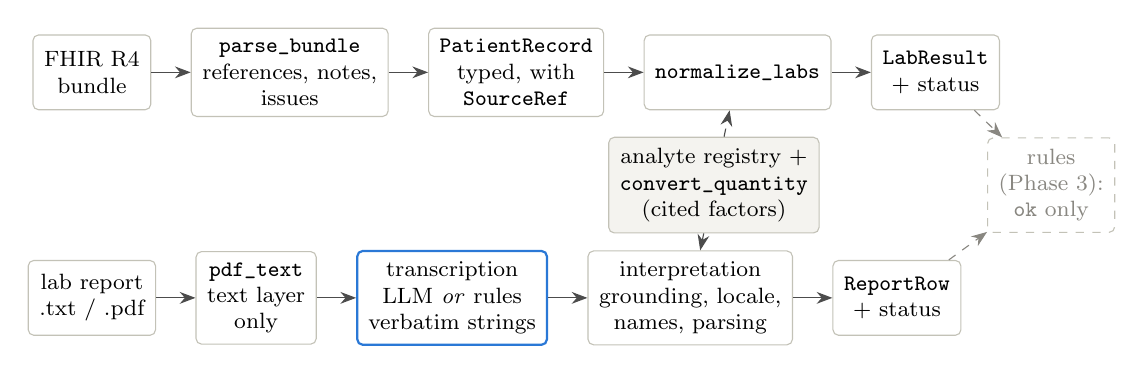
\begin{tikzpicture}[
  font=\footnotesize,
  box/.style={draw=boxline,fill=white,rounded corners=2pt,align=center,inner sep=4pt,minimum height=0.95cm},
  llm/.style={box,draw=medblue,line width=0.8pt},
  code/.style={box},
  shared/.style={box,fill=boxbg},
  later/.style={box,dashed,text=muted},
  arr/.style={-{Stealth[length=2mm]},color=black!70},
  node distance=0.45cm and 0.5cm]
  % FHIR path
  \node[code] (fhir) {FHIR R4\\bundle};
  \node[code,right=of fhir] (parse) {\code{parse_bundle}\\references, notes,\\issues};
  \node[code,right=of parse] (record) {\code{PatientRecord}\\typed, with\\\code{SourceRef}};
  \node[code,right=of record] (norm) {\code{normalize_labs}};
  \node[code,right=of norm] (lab) {\code{LabResult}\\+ status};
  % report path
  \node[code,below=1.9cm of fhir] (rep) {lab report\\.txt / .pdf};
  \node[code,right=of rep] (pdf) {\code{pdf_text}\\text layer\\only};
  \node[llm,right=of pdf] (tr) {transcription\\LLM \emph{or} rules\\verbatim strings};
  \node[code,right=of tr] (interp) {interpretation\\grounding, locale,\\names, parsing};
  \node[code,right=of interp] (row) {\code{ReportRow}\\+ status};
  % shared registry
  \node[shared] (reg) at ($(norm)!0.5!(interp)$) {analyte registry +\\\code{convert_quantity}\\(cited factors)};
  % later phases
  \node[later,right=0.9cm of $(lab)!0.5!(row)$] (rules) {rules\\(Phase 3):\\\code{ok} only};
  \draw[arr] (fhir) -- (parse); \draw[arr] (parse) -- (record); \draw[arr] (record) -- (norm); \draw[arr] (norm) -- (lab);
  \draw[arr] (rep) -- (pdf); \draw[arr] (pdf) -- (tr); \draw[arr] (tr) -- (interp); \draw[arr] (interp) -- (row);
  \draw[arr,dashed] (reg) -- (norm); \draw[arr,dashed] (reg) -- (interp);
  \draw[arr,dashed,color=muted] (lab) -- (rules); \draw[arr,dashed,color=muted] (row) -- (rules);
\end{tikzpicture}
\caption{Data paths built in Phase~1. Only the blue box may use an LLM. It copies strings verbatim, and code checks everything it returns. Dashed boxes are later phases.}
\label{fig:pipeline}
\end{figure}

Table~\ref{tab:modules} gives the responsibilities of the modules. The graph, rules, retrieval and API modules exist only as empty packages for now. Their stated rules on LLM use bind the later phases.

\begin{table}[h]
\centering\small
\begin{tabularx}{\linewidth}{@{}l>{\raggedright\arraybackslash}X>{\raggedright\arraybackslash}p{4.6cm}@{}}
\toprule
Module & Responsibility & LLM allowed? \\
\midrule
\code{ingest} & Parse FHIR bundles and lab reports into typed models, keeping a reference to each source & Only to transcribe reports; the output is schema-checked and grounded \\
\code{normalize} & LOINC mapping, UCUM units and conversions, numbers, dates, reference ranges & No \\
\code{graph} & Per-patient graph with typed edges, and its persistence & No \\
\code{rules} & Guideline criteria as code; flags carry their evidence & No \\
\code{rag} & Retrieval over versioned sources, with citations at chunk level & Embeddings only \\
\code{agent} & Note checks; explanations in two registers and two languages & Language only, grounded in cited chunks \\
\code{api}, \code{gnn} & Endpoints; graph-learning research & No \\
\bottomrule
\end{tabularx}
\caption{Modules and where an LLM may be used (from \code{docs/architecture.md}).}
\label{tab:modules}
\end{table}

%=====================================================================================
\section{Phase 0: engineering foundations and a reproducible cohort}

\subsection{Tooling and quality gates}
The project uses Python~3.12 with \code{uv}, in a \code{src/} layout. Phase~0 set up the quality gates. All of them run through \code{uv}, so they use the locked versions, and \code{make check} runs them all:
\begin{itemize}
  \item \textbf{ruff}, for linting and formatting with a line length of 100. Besides the usual rule sets, two matter here. \texttt{DTZ} forbids timezone-naive datetimes, a classic source of timeline bugs. \texttt{T20} forbids \code{print} in library code, so record values cannot leak to the console.
  \item \textbf{mypy} in strict mode, with the pydantic plugin, over \code{src/} and \code{scripts/}.
  \item \textbf{pytest}. Tests that need external resources are opt-in, through \texttt{--run-llm}, \texttt{--run-synthea} and \texttt{--run-mimic}. MIMIC tests never run in CI.
  \item \textbf{pre-commit} hooks:
  \begin{itemize}
    \item YAML and TOML checks, file hygiene, a 500\,KB limit on added files, and private-key detection;
    \item \code{nbstripout}, which removes notebook outputs before they can be committed;
    \item the ruff and mypy checks above;
    \item a local hook, \code{forbid-data-files}, that blocks data and model file types (\code{.ndjson}, \code{.csv}, \code{.parquet}, \code{.pt}, \code{.pkl}, \code{.jar}, \code{.sqlite}, \code{.pdf}, \ldots) anywhere outside \code{tests/fixtures/} and \code{docs/}.
  \end{itemize}
\end{itemize}
A GitHub Actions workflow runs \code{make check}; it stays inactive until the repository is pushed.

\subsection{Privacy safeguards}
\begin{itemize}
  \item \textbf{Data never lives in the repository.} It lives under \code{MEDGRAPH_DATA_DIR}, on an external SSD. \code{.gitignore} covers the default data location, and the hook above blocks data file types.
  \item \textbf{The LLM stays local.} \code{check_local_llm} runs whenever settings are loaded and refuses two things:
  \begin{itemize}
    \item any endpoint whose host is not the loopback interface;
    \item any Ollama model tagged \texttt{cloud}, because a local Ollama server forwards such models to ollama.com.
  \end{itemize}
  Only \code{MEDGRAPH_ALLOW_REMOTE_LLM=true} overrides the check.
  \item \textbf{Assistant sessions.} The project's working rules (\code{CLAUDE.md}) forbid opening or printing MIMIC data or real personal records in an AI-assistant session: the PhysioNet data use agreement and the GDPR both apply. Debugging uses synthetic fixtures, and only aggregates are shown.
\end{itemize}

\subsection{A reproducible Synthea cohort}
Synthea v4.0.0 runs as a local JAR on JDK~21. Its SHA-256 is checked against the digest GitHub publishes for the release asset. Each cohort is described by a YAML configuration. Each generated cohort gets a \code{MANIFEST.json} recording:
\begin{itemize}[nosep]
  \item the configuration, the exact command and the tool versions;
  \item the git state;
  \item one SHA-256 per file and an order-independent \emph{content digest} over all of them.
\end{itemize}

Two hidden sources of non-determinism turned up and were fixed:
\begin{enumerate}
  \item \textbf{The clock.} In Synthea v4.0.0 the end time of the simulation is taken from the system clock, and the reference-date flag \texttt{-r} does not move it. Both \texttt{-r} and \texttt{-e} are therefore pinned, to 2026-01-01.
  \item \textbf{The time zone.} Synthea formats timestamps in the JVM's default time zone, so they carried \texttt{+01:00} or \texttt{+02:00} offsets depending on the machine. The JVM now runs with \texttt{-Duser.timezone=UTC}, and its locale is pinned to \texttt{en-US}.
\end{enumerate}
Afterwards, the pilot cohort was regenerated twice: once in the machine's time zone (Europe/Rome) and once with \texttt{TZ=America/New\_York}. Both runs gave the same content digest, and every timestamp had offset \texttt{+00:00}. Table~\ref{tab:cohorts} lists the cohorts.

\begin{table}[h]
\centering\small
\begin{tabular}{@{}lrrrrl@{}}
\toprule
Cohort & Patients (deceased) & Size & Generation & Seeds & Content digest \\
\midrule
pilot-10 & 12 (2) & 38\,MB & 9\,s & 42 / 42 & \texttt{0eaba7ec\ldots} \\
dev-1000 & 1,148 (148) & 4.2\,GB & 52\,s & 42 / 42 & \texttt{921e427d\ldots} \\
\bottomrule
\end{tabular}
\caption{Synthea cohorts: reference and end date 2026-01-01, Massachusetts, FHIR R4 (US Core 6.1.0) export, 10 years of exported history per patient. Synthea exports the patients who die during the simulation in addition to the requested living ones. Timings were taken on an Apple M3.}
\label{tab:cohorts}
\end{table}

\paragraph{The external drive.} The data drive is formatted exFAT, which brought two quirks:
\begin{itemize}
  \item macOS writes a \code{._*} AppleDouble companion next to every file. Unfiltered, these broke JSON parsing.
  \item Names containing non-ASCII characters are listed in NFD form but can only be deleted by their NFC spelling.
\end{itemize}
To handle this, all scans go through \code{iter_data_files}, which skips hidden files, and all deletions go through \code{remove_tree}.

\subsection{What the cohort profile showed}
Before any design work, \code{scripts/profile_cohort.py} wrote an aggregate-only profile of dev-1000. Lab codes were found both by expected code \emph{and} by keyword search over display names, so that the profile could reveal codes nobody anticipated. These findings describe the Synthea generator, not any real population. They shaped the design as Table~\ref{tab:profile} shows.

\begin{table}[h]
\centering\small
\begin{tabularx}{\linewidth}{@{}>{\raggedright\arraybackslash}X>{\raggedright\arraybackslash}X@{}}
\toprule
Finding (dev-1000) & Consequence \\
\midrule
eGFR appears only as LOINC \texttt{33914-3}, the MDRD equation, in 25\% of patients. There is no CKD-EPI code. & Rules will compute CKD-EPI 2021 from creatinine, age and sex. A reported eGFR is shown, labelled with its equation, and never used as the sole basis of a flag. \\
That same eGFR code comes in two units: 8,051 values in \texttt{mL/min/\{1.73\_m2\}} (median 53.6) and 3,490 in \texttt{mL/min} (median 22.3). & These units cannot be converted without body surface area. Normalization marks the mismatch instead of converting. \\
Creatinine comes under two codes: \texttt{38483-4} (blood, 44\% of patients) and \texttt{2160-0} (serum or plasma, 15\%). Its maximum is 97.3\,mg/dL. & Both codes are read. Sanity bounds catch values that are physically implausible. \\
The urine albumin/creatinine ratio exists only as \texttt{14959-1}, in 6\% of patients. & Albuminuria criteria can be tested only in this small subgroup. \\
Haemoglobin exists for every patient, with a median of 2 values each. 936 patients have two or more values at least 90 days apart. 33\% have ``Anemia (disorder)'' coded. & Anaemia rules have the longitudinal data they need. Whether the coded anaemia matches the values is a question for Phase~3. \\
CKD stages pile up: earlier stages stay active as later ones are added. & Ingestion keeps clinical status and abatement dates; nothing is collapsed silently. \\
Every encounter has a templated note (median 1,333 characters), stored twice: as a DocumentReference and as a DiagnosticReport's \texttt{presentedForm}. & Notes are deduplicated. Checking whether a note acknowledges a finding is trivial on Synthea, so it needs real annotated notes for evaluation. \\
136 of the 148 deceased patients have an encounter dated after their death. & Ingestion tolerates this and records a warning; it does not reject the record. \\
\bottomrule
\end{tabularx}
\caption{Profile findings and their consequences (\code{docs/data/synthea-dev-1000-profile.md}).}
\label{tab:profile}
\end{table}

%=====================================================================================
\section{Phase 1a: record model and FHIR ingestion}

\subsection{Record model}
All later modules consume one shared record model, built from frozen pydantic~v2 classes in \code{medgraph/records.py}. Its main design choices are these:
\begin{itemize}
  \item \textbf{Provenance on every record.} A \code{SourceRef} holds the SHA-256 of the source file, the resource type and the resource ID.
  \item \textbf{Values exactly as written.} Bundles are parsed with \code{parse_float=Decimal}, so \texttt{1.30} stays \texttt{1.30} and never turns into a binary float. Source values are never overwritten: canonical values sit beside the originals.
  \item \textbf{Honest time.} A \code{Timepoint} holds the calendar date as written and its precision (year, month, day or instant). It holds an absolute instant only when the source gives a timezone offset. A FHIR time of day without an offset is rejected as \code{invalid_time}, never assumed to be local or UTC.
  \item \textbf{Problems are data, not exceptions.} Problems become \code{IngestIssue}s attached to the record: an invalid resource, an invalid time, an unresolved reference, an unexpected reference type, an event after death, an unsupported value or an unsupported attachment. A broken resource is skipped with an error issue, and the rest of the bundle is still read.
\end{itemize}

\subsection{Parser}
\code{parse_bundle} reads these resource types:
\begin{itemize}[nosep]
  \item Patient, Encounter, Condition, MedicationRequest, Observation and Procedure;
  \item DiagnosticReport, for lab panels;
  \item DocumentReference, for notes.
\end{itemize}
The following behaviours matter:
\begin{itemize}[nosep]
  \item References are resolved either by \code{fullUrl} or by \texttt{Type/id}. Conditional references are ignored.
  \item A bundle must contain exactly one Patient.
  \item Identical note text within one encounter becomes a single note that lists every resource carrying it.
  \item Events dated after death raise a warning.
\end{itemize}
Out-of-scope types are counted but not read. In dev-1000 these include 123,164 claims and 16,960 MedicationAdministrations. Monitoring rules will work from prescriptions, and this choice is recorded as revisable.

\paragraph{Evidence.} All 1,148 dev-1000 patients parse, and every in-scope resource is accounted for (opt-in test \code{make test-synthea}). The only issues raised are the 136 known events after death.

%=====================================================================================
\section{Phase 1b: laboratory normalization}

\subsection{Principle: never guess}
Normalization reports anything it cannot read without assuming something:
\begin{itemize}
  \item \textbf{Numbers.} \code{parse_number} handles Italian and English separators. A number whose meaning depends on the locale, such as \texttt{1,234}, is rejected when no locale is given.
  \item \textbf{Dates.} A numeric report date is read day-first or month-first only as the stated locale says.
  \item \textbf{Units.} Unit spellings map to UCUM codes through an explicit synonym table. An unknown spelling is reported.
  \item \textbf{Reference ranges} come only from the source. medgraph never supplies its own.
\end{itemize}

\subsection{Analyte registry}
The registry (Table~\ref{tab:registry}) defines the analytes in scope. For each it gives the LOINC codes, a canonical UCUM unit, the accepted units with their conversion factors, and wide \emph{sanity bounds}. The bounds are engineering limits for catching unit mix-ups and corrupted values. They are not clinical criteria.

Any non-trivial factor must cite its source, and a test enforces this. Two factors are cited:
\begin{itemize}[nosep]
  \item creatinine, $1\,\text{mg/dL} = 88.4\,\mu\text{mol/L}$ (KDIGO 2024 CKD guideline, \emph{Kidney Int} 2024;105(4S));
  \item the albumin/creatinine ratio, mg/mmol to mg/g, via the molar mass of creatinine (113.12\,g/mol).
\end{itemize}
eGFR keeps the equation its LOINC code implies. Values in \texttt{mL/min} are not converted; their status is \code{unit_incompatible}.

\begin{table}[h]
\centering\footnotesize
\begin{tabularx}{\linewidth}{@{}l l >{\raggedright\arraybackslash}X >{\raggedright\arraybackslash}p{2.6cm} r@{}}
\toprule
Analyte & Canonical & LOINC codes & Accepted units & Sanity bounds \\
\midrule
creatinine & mg/dL & 2160-0, 38483-4, 14682-9 & mg/dL, mg/L, \textmu mol/L & 0.05--40 \\
eGFR & mL/min/1.73\,m$^2$ & 33914-3, 48642-3, 48643-1 (MDRD); 62238-1, 88293-6, 88294-4 (CKD-EPI 2009); 98979-8 (CKD-EPI 2021) & as reported only & 1--250 \\
urine ACR & mg/g & 9318-7, 14959-1 & mg/g, \textmu g/mg, mg/mmol & 0--30,000 \\
urine albumin & mg/L & 14957-5, 1754-1 & mg/L, \textmu g/mL, mg/dL & 0--30,000 \\
urine protein & mg/dL & 2888-6, 5804-0, 20454-5 (qualitative) & mg/dL, mg/L, g/L & 0--5,000 \\
haemoglobin & g/dL & 718-7 & g/dL, g/L & 2--25 \\
haematocrit & \% & 4544-3, 20570-8 & \%, L/L & 5--80 \\
MCV & fL & 787-2, 30428-7 & fL, \textmu m$^3$ & 40--150 \\
ferritin & ng/mL & 2276-4 & ng/mL, \textmu g/L & 0.5--100,000 \\
\bottomrule
\end{tabularx}
\caption{Analyte registry (\code{medgraph/normalize/analytes.py}). Bounds are in the canonical unit.}
\label{tab:registry}
\end{table}

Every normalized result carries a status. \code{ok} means converted and within the bounds; only \code{ok} results may feed rules. The other statuses each name a reason, so a flag can later say what it could not use:
\begin{itemize}[nosep]
  \item \code{implausible}: converted, but outside the bounds, so kept and shown but never used;
  \item \code{unit_unknown}: a unit spelling that isn't recognised;
  \item \code{unit_incompatible}: a recognised unit that can't be converted for this analyte;
  \item \code{non_numeric}: a qualitative result;
  \item \code{missing_value}: no value at all.
\end{itemize}

\subsection{Evidence over the whole cohort}
\code{scripts/check_normalization.py} runs the application pipeline over all 1,148 patients (Table~\ref{tab:norm}). Every unit spelling recorded under an in-scope code was recognised, except the dipstick placeholder \texttt{\{presence\}}. Every value marked implausible is a creatinine between 40.4 and 97.3\,mg/dL. The 3,490 eGFR values in \texttt{mL/min} were kept apart, as intended.

\begin{table}[h]
\centering\small
\begin{tabular}{@{}lrrrr@{}}
\toprule
Analyte & \code{ok} & implausible & unit incompatible / unknown & non-numeric \\
\midrule
creatinine (2 codes) & 17,376 & 46 & 0 & 0 \\
eGFR (MDRD) & 8,051 & 0 & 3,490 & 0 \\
urine ACR & 2,093 & 0 & 0 & 0 \\
urine protein (2 codes) & 7,844 & 0 & 163 & 7,708 \\
haemoglobin & 3,358 & 0 & 0 & 0 \\
haematocrit (2 codes) & 3,358 & 0 & 0 & 0 \\
MCV (2 codes) & 3,351 & 0 & 0 & 0 \\
ferritin & 372 & 0 & 0 & 0 \\
\bottomrule
\end{tabular}
\caption{Normalization outcomes on dev-1000 (\code{docs/data/synthea-dev-1000-normalization.md}).}
\label{tab:norm}
\end{table}

%=====================================================================================
\section{Phase 1c: a synthetic lab-report benchmark}

\subsection{Requirements}
Evaluating extraction on synthetic text carries its own risks. Each of the following requirements guards against a specific way the numbers could be inflated:
\begin{enumerate}
  \item \textbf{No LLM writes the reports.} If a model, or a related one, wrote the text it is tested on, it could exploit its own phrasing. The reports are therefore printed by code templates.
  \item \textbf{Exact ground truth.} The truth file holds the exact printed string of every field, so scoring needs no fuzzy matching. The \emph{canonical} truth value is computed from the printed value with the registry's factors.
  \item \textbf{Held-out layouts and names.} The test split contains layouts and analyte names that development never shows. Generalization is measured, not assumed.
  \item \textbf{Patient-disjoint splits.} Each patient is assigned to a split by a hash.
  \item \textbf{Text and PDF} versions of every report.
\end{enumerate}

\subsection{Generation}
\code{scripts/generate_lab_reports.py} builds each report from one day of a dev-1000 patient's real (Synthea) lab values:
\begin{itemize}
  \item \textbf{Tests.} A catalog of 23 printable tests: blood count, chemistry, lipids, HbA1c, ferritin and urine tests. Eight map to the registry; the rest are realistic out-of-scope rows. A report prints at most 15 rows, in-scope tests first.
  \item \textbf{Styles.} There are three printing styles:
  \begin{itemize}
    \item \textbf{Italian}: decimal comma and day-first dates;
    \item \textbf{en-GB}: SI units and day-first dates. Creatinine is printed in \textmu mol/L (factor 88.4), haemoglobin in g/L, haematocrit in L/L and ACR in mg/mmol;
    \item \textbf{en-US}: conventional units and month-first dates.
  \end{itemize}
  About 30\% of collection dates are written out in words (``16 settembre 2025'').
  \item \textbf{Analyte names.} 100 seen names and 40 held-out names, in both languages. On the test split each eligible row uses a held-out name with probability 0.5.
  \item \textbf{Reference ranges} are printed for realism. They are \textbf{illustrative test data, not cited clinical ranges}, and medgraph never uses printed ranges as criteria.
  \item \textbf{Synthetic marking.} Every report's header names a synthetic laboratory and marks the report as synthetic, for testing only.
  \item \textbf{PDFs.} PDFs are rendered with ReportLab in a monospace font, with invariant output, and carry a text layer.
\end{itemize}

\subsection{Layout families}
There are six families, printed with the same values. The first four are used for development and test; \texttt{two\_column} and \texttt{narrative} appear only in the test split:

\begin{Verbatim}[label={\scriptsize table (en-US)}]
  TEST                         RESULT     UNITS             REFERENCE RANGE        FLAG
  HGB                          17.2       g/dL              12.0 - 15.5            H
\end{Verbatim}
\begin{Verbatim}[label={\scriptsize dotted (it)}]
  Leucociti ........................  7,22    10^3/µL          (4,0 - 10,0)
\end{Verbatim}
\begin{Verbatim}[label={\scriptsize colon (en-GB)}]
Hemoglobin: 130 g/L (ref 130 - 170)
\end{Verbatim}
\begin{Verbatim}[label={\scriptsize sections (it)}]
CHIMICA CLINICA
  Creatinina                      1,33      mg/dL            [0,70 - 1,20]        H
    metodo: fotometrico
\end{Verbatim}
\begin{Verbatim}[label={\scriptsize two\_column (en-GB), held out}]
  Serum creatinine  283 µmol/L  [44 - 80] H  eGFR  82 mL/min  [> 60]
\end{Verbatim}
\begin{Verbatim}[label={\scriptsize narrative (it), held out}]
Risultati degli esami: Glucosio 83 mg/dL (riferimento 70 - 99). BUN 10 mg/dL
(riferimento 7 - 20). Creatininemia 2,99 mg/dL (riferimento 0,70 - 1,20), alto.
\end{Verbatim}

The narrative layout wraps lines anywhere, even inside a range (\texttt{136 -} / \texttt{145}). This is why the grounding check (Section~\ref{sec:interp}) normalizes whitespace before matching.

\subsection{The report set}
\begin{table}[h]
\centering\small
\begin{tabularx}{\linewidth}{@{}l>{\raggedright\arraybackslash}Xrrr@{}}
\toprule
Split & Families & Reports & Rows per format & Held-out-name rows \\
\midrule
development & colon, dotted, sections, table & 24 & 186 & 0 \\
test & the same four, plus two\_column and narrative (held out) & 48 & 405 & 52 \\
\bottomrule
\end{tabularx}
\caption{\texttt{reports-v1}: seed 7, half of the patients assigned to the test split. Each language has its own cell per family: 3 reports per cell in development and 4 in test. Content digest \texttt{e47d7ca5\ldots}, 216 files.}
\label{tab:reports}
\end{table}

%=====================================================================================
\section{Phase 1d: extraction pipeline}

\subsection{Two stages}
Extraction is split so that the LLM never makes a decision that matters medically.

\paragraph{Stage 1: transcription.} For each result row, the LLM copies five fields as \emph{verbatim strings}:
\begin{itemize}[nosep]
  \item the analyte name;
  \item the value;
  \item the unit;
  \item the reference range;
  \item the flag.
\end{itemize}
It also copies the collection date. The output is forced to a JSON schema through Ollama's structured output, and decoding is deterministic: temperature~0, seed~42, thinking off, a 4,096-token context. The model is \texttt{qwen3.5:9b}, quantized to Q4\_K\_M and served locally by Ollama. The prompt is versioned; Appendix~\ref{app:prompt} gives the final version.

\paragraph{Stage 2: interpretation.}\label{sec:interp} Deterministic code takes over, in order:
\begin{enumerate}
  \item \textbf{Grounding check.} Every transcribed field must occur in the report text, with whitespace normalized. A row that fails is \code{ungrounded}: it is kept for review and never used. This is the defence against invented values.
  \item \textbf{Locale detection.} The language is chosen by counting Italian and English vocabulary. An English report counts as en-GB when SI units appear, and as en-US otherwise. Section~\ref{sec:limits} discusses the risks of this heuristic.
  \item \textbf{Name mapping} through an explicit Italian/English table of 53 names, after normalizing case, accents and trailing punctuation. One trailing parenthetical may be dropped (``Ferritin (serum)''). An unknown name is \code{unmapped}; the system never guesses which test a row is.
  \item \textbf{Value/unit separation.} When the model copies the unit into the value field (\texttt{"130 g/L"}), code splits it off. Both parts must still be grounded.
  \item \textbf{Parsing and conversion}, using the same functions and registry as for FHIR labs.
\end{enumerate}
A report row ends with one of these statuses:
\begin{itemize}[nosep]
  \item the FHIR statuses: \code{ok}, \code{implausible}, \code{unit_unknown}, \code{unit_incompatible} and \code{non_numeric};
  \item \code{unparseable_value}, \code{unmapped} and \code{ungrounded}.
\end{itemize}

\paragraph{Rule-based baseline.} Regular expressions were written for the development layouts:
\begin{itemize}[nosep]
  \item a date line;
  \item colon rows;
  \item dot leaders;
  \item cells separated by two or more spaces.
\end{itemize}
The baseline goes through the same interpretation stage, so the LLM must beat it to justify its cost.

\paragraph{PDF text.} Only PDFs with a text layer are accepted. A PDF without one raises \code{NoTextLayerError} instead of being run through OCR silently. Lines are rebuilt from word positions. A horizontal gap wider than 1.5 average character widths becomes a column break. This replaced pdfplumber's layout mode, which merged adjacent columns.

%=====================================================================================
\section{Evaluation methodology}

\subsection{Protocol}
\begin{itemize}
  \item The prompt and the rules were tuned on the \textbf{development split only}.
  \item The prompt was frozen at version~3 \textbf{before} the test split was run.
  \item The test split was run once, and its results are reported as they came out.
  \item A new prompt version would get a new test run; no choice is made among several runs.
\end{itemize}

\subsection{Matching and metrics}
Transcribed rows are paired with truth rows by normalized analyte name, in order. Table~\ref{tab:metrics} defines the metrics. Two of them matter most for safety:
\begin{itemize}
  \item \textbf{End-to-end canonical value}: what fraction of in-scope rows reached rules with the right number;
  \item \textbf{Wrong values accepted}: what fraction of accepted rows carry a wrong number.
\end{itemize}

\begin{table}[h]
\centering\small
\begin{tabularx}{\linewidth}{@{}l>{\raggedright\arraybackslash}X@{}}
\toprule
Metric & Definition (numerator / denominator) \\
\midrule
row recall / precision & matched rows / truth rows; matched rows / transcribed rows \\
value, unit, range, flag exact & transcribed field equals the printed string (whitespace-normalized; range labels ignored) / matched rows \\
end-to-end canonical value & in-scope truth rows whose interpreted row has the right analyte and canonical value (status \code{ok} or \code{implausible}) / in-scope truth rows \\
\quad split by name & the same, for rows printed under seen names and under held-out names \\
ungrounded rows & rows rejected by the grounding check / transcribed rows \\
wrong values accepted & \code{ok} rows whose analyte or value disagrees with the truth, or which match no truth row / \code{ok} rows \\
name mapping & transcribed names mapped to the right analyte / matched in-scope rows, for seen and for held-out names \\
collection date, locale & correct / reports \\
\bottomrule
\end{tabularx}
\caption{Metrics (\code{scripts/evaluate_extraction.py}).}
\label{tab:metrics}
\end{table}

\subsection{Uncertainty}
Rows within one report share their errors, so 95\% intervals are \textbf{bootstrapped over reports}: 1,000 resamples, percentile method.

At an observed rate of 0\% or 100\%, every resample gives the same rate, so the bootstrap interval collapses to a point and overstates certainty. In those cases the exact Clopper--Pearson interval on the pooled count is used instead. These intervals are marked $^*$ in the tables. They treat rows as independent, which is optimistic when errors cluster. All interval bounds are rounded outwards.

\subsection{Reproducibility and provenance}
\begin{itemize}
  \item \textbf{What is cached.} Only the LLM's transcription is cached. It is reused only when all of these match:
  \begin{itemize}[nosep]
    \item the hash of the report text;
    \item the model name and the model digest;
    \item the prompt version;
    \item the context size.
  \end{itemize}
  Interpretation and scoring are recomputed with the current code every time. The rules are never cached.
  \item \textbf{What every results file records:}
  \begin{itemize}[nosep]
    \item the report-set digest;
    \item the git commit, with a flag for uncommitted changes;
    \item a digest of the code that determines the results;
    \item the model digest.
  \end{itemize}
  Results were produced before the code was committed, so the commit alone would not identify the code.
  \item \textbf{Truncation check.} Ollama silently truncates input that overflows the context, so context use was checked on every run.
  \begin{itemize}[nosep]
    \item Prompt plus output peaked at 1,623 tokens (development, v2), 1,490 (development, v3) and 1,700 (test).
    \item The server reported \texttt{truncated = 0} on every request.
  \end{itemize}
\end{itemize}

%=====================================================================================
\section{Results}

\subsection{Development split: prompt iteration}
Table~\ref{tab:dev} and Figure~\ref{fig:dev} compare the two prompt versions with the rules.

\begin{table}[h]
\centering\small
\begin{tabular}{@{}lrrr@{}}
\toprule
Development split, text (24 reports, 186 rows) & rules & LLM, prompt v2 & LLM, prompt v3 \\
\midrule
row recall & 98.9\% & 100\% & 100\% \\
value exact & 100\% & 83.3\% & 91.9\% \\
range exact & 100\% & 96.8\% & 100\% \\
ungrounded rows (rejected) & 0\% & 5.4\% & 0\% \\
\textbf{end-to-end canonical value} & \textbf{100\%} & \textbf{90.0\%} (77--100) & \textbf{100\%} (94--100$^*$) \\
\bottomrule
\end{tabular}
\caption{Development results. Prompt v2's intervals predate the exact-interval rule; its name-mapping figure was rescored with the corrected metric (Section~\ref{sec:log}).}
\label{tab:dev}
\end{table}

\begin{figure}[h]
\centering
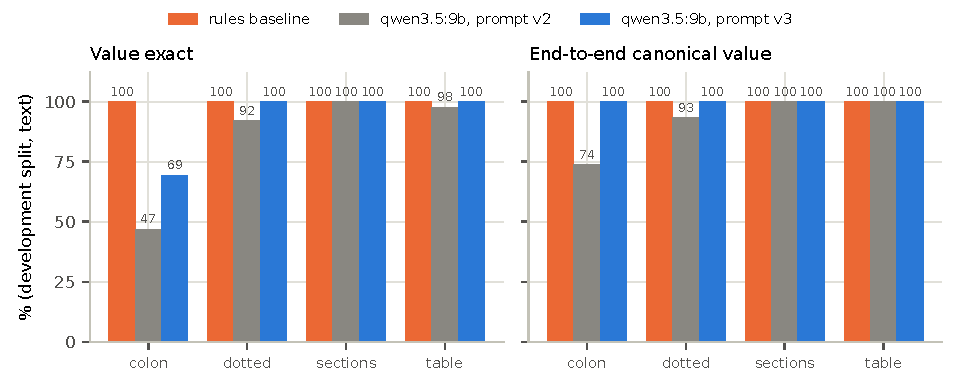
\includegraphics[width=\linewidth]{figures/extraction-dev-prompts.pdf}
\caption{Development split, per layout family. Prompt v2 lost values on the colon layout. Version~3 fixed end-to-end recall; on en-US colon reports the model still copies units into the value field, which code repairs.}
\label{fig:dev}
\end{figure}

\paragraph{What prompt v2 got wrong.} Row recall was 100\%. Every loss came from fields that weren't split apart:
\begin{itemize}
  \item \textbf{21 rows: unit and range copied into the value}, all in English colon-layout reports (\texttt{"7.4 x10\^{}9/L (ref 4.0 - 10.0)"}). Code splits off a bare unit (en-US), but not a unit followed by a range (en-GB).
  \item \textbf{10 rows: a flag turned into a value prefix}, always on rows flagged abnormal. The model produced \texttt{">3,76"} for a printed \texttt{3,76 \ldots\ *} and \texttt{"* 3,64"} when the asterisk was printed at the end of the line. \textbf{The grounding check rejected all ten}, so no invented comparator reached the output. That is the designed safety behaviour; recall paid the cost.
\end{itemize}

\paragraph{What changed in prompt v3.} The prompt now:
\begin{itemize}[nosep]
  \item asks for five \emph{separate} fields;
  \item forbids a unit, range or flag in the value field;
  \item states that a flag is not a comparator;
  \item adds one worked example, written in the colon layout (a development family).
\end{itemize}
End-to-end recall rose to 100\% with no rows rejected. \textbf{That figure is measured on the split the prompt was tuned on, so it is not an estimate.}

\subsection{Test split: the held-out estimate}
Table~\ref{tab:test} gives the main results; Figure~\ref{fig:test} breaks them down by layout family.

\begin{table}[h]
\centering\footnotesize
\begin{tabular}{@{}lrrr@{}}
\toprule
Test split (48 reports, 405 rows) & LLM, text & LLM, PDF & rules, text \\
\midrule
row recall & 99.8\% (99--100) & 99.8\% (99--100) & 67.9\% (53--81) \\
\quad on the held-out layouts & 100\% & 100\% & 0\% \\
value exact & 94.8\% (89--100) & 95.3\% (89--100) & 100\%$^\dagger$ \\
\textbf{end-to-end, seen names} & \textbf{100\%} (94--100$^*$), 66/66 & 66/66 & 69.7\% (52--85), 46/66 \\
\quad on the held-out layouts & 20/20 & 20/20 & 0/20 \\
end-to-end, held-out names & 5.9\% (0--14), 3/51 & 3/51 & 3/51 \\
end-to-end, all in-scope rows & 59.0\% (48--70) & 59.0\% & 41.9\% (30--54) \\
ungrounded rows (rejected) & 0\% (0--1$^*$) & 0\% & 0\% \\
\textbf{wrong values accepted} & \textbf{0 of 69} (0--6$^*$) & 0 of 69 & 0 of 49 (0--8$^*$) \\
collection date, locale & 100\% (92--100$^*$) & 100\% & 100\% \\
\bottomrule
\end{tabular}
\caption{Test results, prompt v3, single run. $^*$~exact binomial interval. $^\dagger$~over the rows the rules matched, which exclude the held-out layouts.}
\label{tab:test}
\end{table}

\begin{figure}[h]
\centering
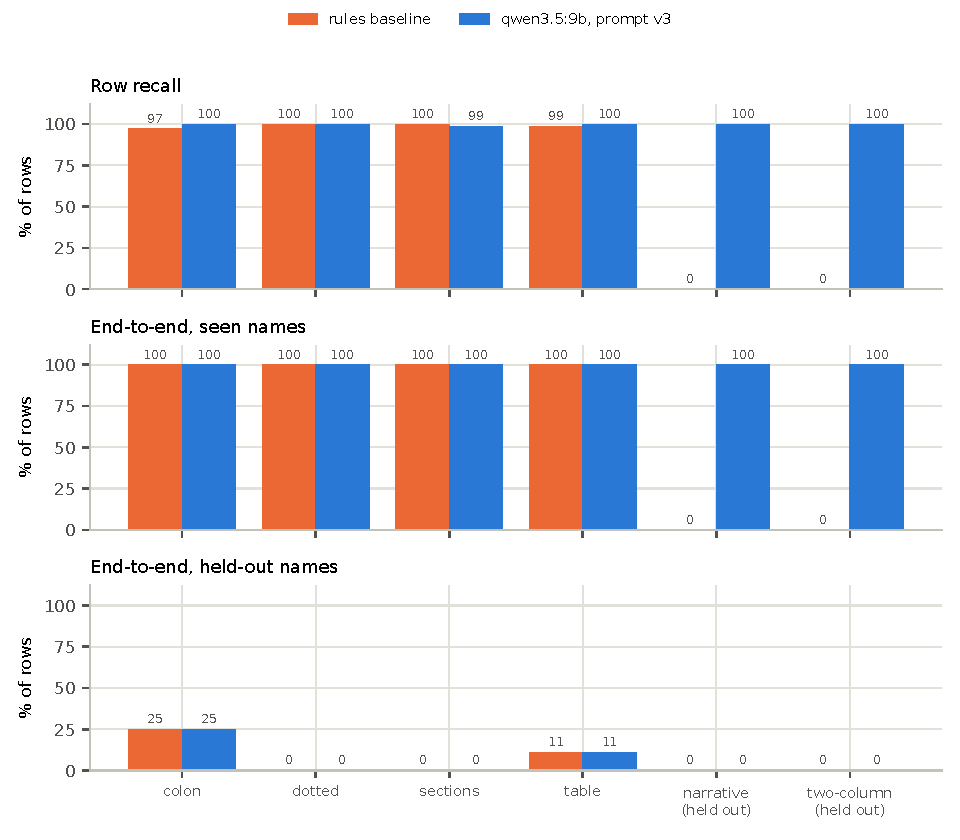
\includegraphics[width=0.92\linewidth]{figures/extraction-test-by-family.pdf}
\caption{Test split by layout family (text). The rules read none of the held-out layouts. The LLM delivered every in-scope value printed under a known name. On held-out names both methods share the same name table, so they score the same by design.}
\label{fig:test}
\end{figure}

\paragraph{Reading the results.}
\begin{itemize}
  \item \textbf{Extraction generalized to unseen layouts.} Every in-scope value printed under a known name was delivered correctly, 20 of them on the two held-out layouts. The PDF results match the text results exactly.
  \item \textbf{The 59\% overall figure measures the name table, not the LLM.} Analyte identity is decided by code. Of the 51 in-scope rows printed under held-out names, 48 were refused as \code{unmapped}; the other three mapped only through the parenthetical rule. A refusal is safe: the row stays visible as \code{unmapped} and is never guessed.
  \item \textbf{Safety.} No wrong value was accepted, in text or in PDF. With 69 accepted rows, the data are compatible with a true rate of up to about 6\%. Ruling out rarer failures needs more data (Section~\ref{sec:limits}).
  \item \textbf{By language} (text): Italian end-to-end 65.5\%, English 52.5\%. The difference follows the share of in-scope rows under held-out names, 51\% in English (30 of 59) against 36\% in Italian (21 of 58). It does not reflect transcription quality, although value exactness was 98.6\% in Italian and 90.5\% in English.
\end{itemize}

\subsection{Error analysis on the test split}
These errors were categorised \emph{after} the frozen run. The pipeline was not changed in response:
\begin{itemize}
  \item \textbf{19 rows: unit copied into the value} (en-US colon and two-column, en-GB narrative). Five were in-scope rows under known names, and code split the unit off correctly in all five. Four had held-out names, and ten were out of scope.
  \item \textbf{2 rows: a narrative flag dropped} (\texttt{low}).
  \item \textbf{1 row missed}, on a sections layout.
  \item \textbf{2 rows: reference range copied as the value.} In one Italian report the model wrote \texttt{< 200} for \texttt{Colesterolo totale: 214 mg/dL (rif. < 200)}, and \texttt{> 40} for HDL cholesterol. The PDF version of the same report was correct.
\end{itemize}

The range-as-value error is the most important finding. The grounding check \emph{cannot} catch it, because the text really is on the page. Both rows were out of scope, so nothing wrong was accepted. On creatinine or haemoglobin, though, \texttt{< 200} would have been accepted as a censored value. One-sided ranges like this are common in real reports. A consistency check is the obvious fix: reject a row whose value equals its range or occurs only inside it. Because the failure was found on the test split, adding the check now would contaminate the test set. It needs a fresh report set before any number can be claimed for it.

\subsection{Cost}
The median was 67\,s per report (maximum 127\,s), with 434 output tokens per report. The 96 test transcriptions took about two hours on an Apple M3 with 16\,GB of RAM. Another CPU-heavy job was running on the machine at the time, so timings are indicative only. Accuracy is unaffected, because decoding is deterministic.

%=====================================================================================
\section{Engineering log: problems found and fixed}
\label{sec:log}
Several of these problems would have inflated results or broken traceability if left alone. They are recorded here because they change how the numbers should be read.

\begin{table}[h]
\centering\footnotesize
\begin{tabularx}{\linewidth}{@{}>{\raggedright\arraybackslash}p{4.4cm}>{\raggedright\arraybackslash}X>{\raggedright\arraybackslash}p{4.2cm}@{}}
\toprule
Problem & Risk & Fix \\
\midrule
Synthea's end time came from the wall clock; timestamps used the machine's time zone & Cohorts not reproducible & Pin \texttt{-r} and \texttt{-e}; JVM in UTC, \texttt{en-US} \\
exFAT AppleDouble files; NFD/NFC deletion & Corrupt reads; failed cleanup & \code{iter_data_files}, \code{remove_tree} \\
Running tests next to the model exhausted 16\,GB and crashed the session & Lost runs & LLM runs go alone; context 4,096 \\
The MLX build of the model failed to load (missing embedding weight) & No faster build to use & Stay on the slower GGUF build \\
Ollama's model folder, set through \texttt{launchctl}, is lost on reboot & Runs fail with HTTP 404 & A private \code{ollama serve} with an explicit model folder (\code{make extract-llm}) \\
A run was killed from outside after 10 reports (cause undetermined; the machine was short of memory and disk) & Lost work & The job runs in its own session and resumes from cached transcriptions \\
Results recorded a commit that contained none of the extraction code & Results not traceable & Git dirty flag, plus a digest of the code that determines results \\
Saved predictions were reused by report ID and prompt version only & Stale or mixed results & Cache key includes text hash, model digest and context size; interpretation always recomputed \\
Name mapping counted a row rejected for its value as a mapping failure & Misattributed errors (v2 development: 95.2\% instead of 100\%) & Score the transcribed name on its own; rules results unchanged \\
Bootstrap intervals collapsed at 0\% and 100\% (``100--100'') & Overstated certainty & Exact Clopper--Pearson at the boundaries, rounded outwards \\
The review notebook's error list mixed predictions from two prompt versions & Wrong counts & Read only the current runs \\
\bottomrule
\end{tabularx}
\caption{Problems found during Phases 0--1.}
\end{table}

\noindent Every refactor of the scoring code was checked against the previous run: the rules baseline's per-report scores were identical before and after each change.

%=====================================================================================
\section{Limitations and threats to validity}
\label{sec:limits}
\begin{enumerate}
  \item \textbf{Synthetic data throughout.} Synthea's labs follow hand-written disease modules. The reports are clean templates: no scanning noise, no handwriting, no tables broken across pages, no logos. Every figure here is an \emph{upper bound} for real reports.
  \item \textbf{``Held out'' means unseen while tuning, not independent.} The held-out layouts and names were written by the same author as the development ones, and the rules baseline was written knowing the development layouts.
  \item \textbf{Small numbers.}
  \begin{itemize}[nosep]
    \item The key safety result rests on 69 accepted rows.
    \item The generalization result rests on 20 in-scope rows on held-out layouts.
    \item The exact intervals assume independent rows, which is optimistic.
  \end{itemize}
  \item \textbf{A single model, a single run.} Decoding is deterministic, so run-to-run variance was not measured. Outputs may still differ across Ollama versions, quantizations and hardware.
  \item \textbf{The locale heuristic is right by construction.} en-GB is inferred from SI units, and the generator ties SI units to en-GB, so 100\% locale detection is expected rather than earned. In real reports a wrong guess has two effects:
  \begin{itemize}
    \item \textbf{Dates:} an ambiguous date such as \texttt{03/04/2025} would be read with day and month swapped.
    \item \textbf{Numbers:} a single separator followed by exactly three digits (\texttt{1.200}) would be read as 1.2 instead of 1200, or the other way round. Sanity bounds catch that factor of 1,000 for creatinine, but not for ferritin, whose bounds are 0.5--100,000.
  \end{itemize}
  This sits uneasily with the ``never guess'' principle. An ambiguous date or number under an \emph{inferred} locale should become an issue, not a guess.
  \item \textbf{Grounding is necessary but not sufficient.} It catches invented text, but not genuine text placed in the wrong field (the range-as-value error).
  \item \textbf{PDF results are optimistic.} All PDFs come from one renderer, in one monospace font, and the column-gap rule was developed on them. Real PDFs vary far more.
  \item \textbf{Timings were confounded} by other work running on the machine at the same time.
\end{enumerate}

%=====================================================================================
\section{Open decisions and next steps}
\begin{enumerate}
  \item \textbf{Range-as-value guard} (recommended first). Add the consistency check, generate a fresh report set with a new seed and new patients, and run one more evaluation of about two hours. Do this before report extraction feeds the graph.
  \item \textbf{Ambiguity under an inferred locale.} Treat ambiguous dates and three-digit-group numbers as issues whenever the locale was inferred rather than declared.
  \item \textbf{Unknown analyte names.} Either grow the tested name table by hand, or let the LLM \emph{propose} a mapping that a person confirms before it is used. The second fits the Phase~5 interface.
  \item \textbf{eGFR equation from reports.} A report row keeps the printed name (``VFG (stima MDRD)'') but has no equation field, unlike FHIR results. Rules will recompute CKD-EPI 2021 from creatinine regardless.
  \item \textbf{Phase~2} (after review): the patient knowledge graph and timeline, beginning with the choice of persistence layer, which is the user's decision.
\end{enumerate}

\appendix
%=====================================================================================
\section{Reproducing the results}
All commands run from the repository root, with \code{MEDGRAPH_DATA_DIR} pointing at the data drive.
\begin{Verbatim}
make setup                         # uv sync + pre-commit hooks
make check                         # ruff, mypy --strict, pytest (330 tests + 1 opt-in)
make synthea-dev                   # dev-1000 cohort (digest 921e427d...)
make profile && make normalization # the two data reports in docs/data/
uv run python scripts/generate_lab_reports.py configs/lab_reports/reports-v1.yaml
make extract-rules SPLIT=dev && make extract-rules SPLIT=test
make extract-llm SPLIT=dev ARGS="--formats text" OLLAMA_MODELS=/Volumes/T7/ollama-models
make extract-llm SPLIT=test OLLAMA_MODELS=/Volumes/T7/ollama-models   # about 2 h
make report                        # figures from metrics.json, then this PDF
make review                        # re-run notebooks/review.ipynb
\end{Verbatim}
The results documents are in \code{docs/results/}, the decisions in \code{docs/decisions/0001}--\code{0003}, and the per-report predictions and metrics under \code{$MEDGRAPH_DATA_DIR/runs/extraction/}.

\section{Code and tests}
The library has 2,028 lines in \code{src/medgraph}; the scripts have 2,800 lines. There are 331 tests: 330 run by default, and one opt-in test parses the whole cohort. They include:
\begin{itemize}[nosep]
  \item property-based round trips (Hypothesis) for every unit conversion and for numbers formatted in Italian and English;
  \item FHIR fixtures written by hand;
  \item an HTTP mock of the Ollama API;
  \item the generator's invariant that each truth string is printed verbatim, in text and in PDF;
  \item tests of the scoring, the cache rules and the exact intervals.
\end{itemize}

\section{Transcription prompt, version 3}
\label{app:prompt}
\begin{Verbatim}
You transcribe laboratory reports into JSON.
For every test result in the report, output one row with five separate fields:
- analyte: the test name exactly as printed
- value: the result only: the number exactly as printed, with its original decimal
  separator, or words such as "Negative". Copy a < or > sign only if it is printed
  directly before the number. Never put a unit, a reference range or a flag in value.
- unit: the unit exactly as printed, or "" if there is none
- reference_range: the reference interval exactly as printed, or ""
- flag: the abnormality marker exactly as printed (for example H, L, * or an arrow),
  or "". A flag is not a < or > sign, and it never goes in value.
Also output collection_date: the specimen collection date exactly as printed, or "".
Example: the line "Sodium: 141 mmol/L (ref 135 - 145) H" becomes analyte "Sodium",
value "141", unit "mmol/L", reference_range "135 - 145", flag "H".
Copy characters exactly. Do not translate, convert units, compute, correct or reorder
anything, and do not add rows that are not in the report. Skip headers, addresses,
comments and method notes.
\end{Verbatim}
The output is forced to a JSON schema: an object with \code{collection_date} and \code{rows}. Each row has the five string fields, all required.

\end{document}
